\documentclass[12pt]{article}
\usepackage{amsmath}
\usepackage{amssymb}
\usepackage{geometry}
\usepackage{enumerate}
\usepackage{natbib}
\usepackage{float}%稳定图片位置
\usepackage{graphicx}%画图
\usepackage[english]{babel}
\usepackage{a4wide}
\usepackage{indentfirst}%缩进
\usepackage{enumerate}%加序号
\usepackage{multirow}%合并行
\title{\large UM-SJTU JOINT INSTITUTE\\DISCRETE MATHEMATICS\\(VE203)\\\ \\\ \\\ \\\ \\\ \\\ \\\ \\\ \\\ \\\ \\\
ASSIGNMENT 3\\\ \\\ \\\ \\\ \\\ \\\ }
\author{Name: Pan Chongdan\\ID: 516370910121}
\date{Date: \today}


\begin{document}
\maketitle
\newpage
\section{Q1}
Assume $A=\{x\in L|x\preceq f(x)\}$, then $\forall x\in A,x\preceq f(x)\preceq f(f(x))$. Let $y=\vee A\Rightarrow f(y)=\vee A\Rightarrow y=f(y)$ Since $X\subseteq A$,$y$ is the greatest upper bound in $X$. Similarly, there exists $z$ is the least lower bound in $X$.
\par $\forall i\in I(x_i\in f(x))$,let $B=\{x\in L|\forall i\in I(x_i\preceq f(x)\preceq x)\}.$
Assume $u=\wedge B,\forall x\in B,u\preceq x\Rightarrow f(u)\preceq f(x)\preceq x\Rightarrow f(u)\preceq u$.
\par $\forall x_i$ which is the lower bound of $B,x_i\preceq u,x_i\preceq u\Rightarrow x_i=f(x_i)\preceq f[f(u)]\preceq f(u)\preceq u,\therefore u\in B\Rightarrow u\preceq f(u)\Rightarrow u=f(u)\Rightarrow u\in X.\forall x_i,u$ is the least upper bound,similarly, we can find the greatest lower bound,so $(x,\preceq)$ is a complete lattice. 
\par$f=2xsin(8x)$, it has 4 points of intersection with the graph of $y=x$ during the interval [0,1].
\begin{figure}[H]
\centering
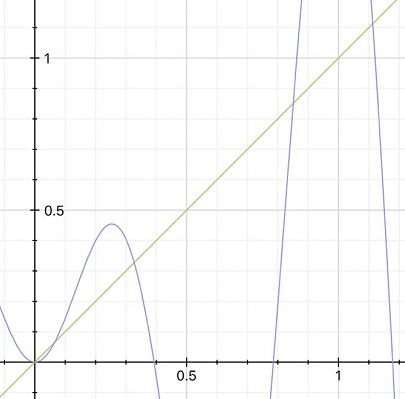
\includegraphics[scale=0.75]{P1.jpg}
\end{figure}
\section{Q2}
Let $f:\mathbb{N}\times\mathbb{N}\rightarrow\mathbb{N}$ defined by 
$$f(x,y)=x^2+2y(x\geq y)$$
$$f(x,y)=2x+1+y^2(x<y)$$
So $f(0,0)=0,f(1,0)=1,f(0,1)=2,f(1,1)=3,f(2,0)=4,f(2,1)=5...$
\\$\therefore$ f is an injection and $|\mathbb{N}\times\mathbb{N}|\leq|\mathbb{N}|$ and $\mathbb{N}\times\mathbb{N}$ is countable.
\par Since Cantor function Function is bijection,so its inverse function satisfies $|\mathbb{N}\times\mathbb{N}|\geq|\mathbb{N}|$ 
$\therefore|\mathbb{N}\times\mathbb{N}|=|\mathbb{N}|$ 
\section{Q3}
\begin{enumerate}[(i)]
\item Since every natural number has a unique factorisation into primes, assume $f={(0,a_0),(1,a_1)...(n,a_n)}$. n means the $(n+1)_{th}$ prime and $a_n$ is (n+1)'s power-1.
\\For example, assume $f={(0,0),(1,1)}\rightarrow 2^{(0+1)}*3^2=18$,so there exists a function g:$S\rightarrow\mathbb{N}\setminus\{0,1\},$which is countable because $\mathbb{N}\setminus\{0,1\}\subset\mathbb{N}$.
$\therefore S$ is countable and $|S|\leq|\mathbb{N}|$.
\par There also exists a injection from $\mathbb{N}\rightarrow S,n\rightarrow\{(0,0),(1,1),(2,2)...(n,n)\}$, so $|\mathbb{N}|=|S|$  
\item $f\preceq_1 f$ because $\forall i\in A((f(i)=f(i))\wedge([n]=[n])),\therefore (S,\preceq)$ is symmetric.
\par Assume $f\preceq_1 g$ and $\forall i\in A((f(i)=g(i))\wedge([n]\preceq_1[m]))$, it's clearly $g\npreceq_1 f$ because $\forall i\in A((f(i)=g(i))$and$([n]\nsubseteq[m]))$.
\\Assume $f\preceq_1 g$ and $(\exists i\in A)(f(i)<g(i)\wedge(\forall j<i)(f(i)=g(j)))$ then the $i_g$ satisfying $g\preceq f$ is bigger than $i$, but $g(i)\neq f(i)\therefore (S,\preceq_1)$ is antisymmetric.
\par Assume $(f\preceq_1 g$ with $j=j_1)\wedge(g\preceq_1 h$ with $j=j_2)$ and $h:[k]\rightarrow \mathbb{N}$,then$f\preceq_1 h$ with $j_=$min$\{j_1,j_2\}\therefore(S,\preceq_1)$ is transitive and it's a partial order.
\\It's a linear order as long as we choose $i$ as 0, then $\forall f,g$ has such relationship.
\\It;s also a well order because I can find the least element as $\{(0,0)\}$
\\It's not a chain complete or a lattice because $f=\{(0,1),(1,2),(2,5)\},g=\{(0,5),(1,3),(2,4)\}$\\$,{f,g}$ doesn't have a upper bound.
\item$\because (f(i)=f(i))\wedge ([n]=[n])\therefore f\preceq_2 f$
\\Assume $(f\preceq_2 g)\wedge([n]\subset[m])$ then $g\npreceq_2 g$ because $[m]\nsubseteq[m]$.
\\Assume $f\preceq_2 g$ and $g\preceq_2 h:[k]\rightarrow \mathbb{N}$ then $f\preceq_2 h$ because $([n]\subseteq[m]\subseteq[k])\wedge(f(i)\leq g(i)\leq h(i))$
\\$\therefore (S,\preceq_2)$ is a partial order.
\\It's not a linear order if $f={(0,1),(1,5)},g={(0,5),(1,2)}$ then they have no relationship.
\\It's not a chain complete because the chain may not have a upper bound.
\\$\forall f,g\in S,f=\{(0,a_0),(1,a_1)...(n,a_n)\}$ and $g=\{(0,b_0),(1,b_1)...(m,b_m)\}$.\\Let $c_n=$max$(a_n,b_n)$,$d=$max$(m,n)$, then $h=\{(0,c_0),(1,c_1)...(d,c_d)\}$ is the least upper bound.
\\Similarly, I can find the greatest lower bound,so it's a complete lattice.
\end{enumerate}
\section{Q4}
$$f(x,y,z)=\frac{1}{2}(\pi(x,y)+z)(\pi(x,y)+z+1)+z$$
\section{Q5}
\begin{enumerate}[(i)]
\item
$\forall A,B,C\in X,A\subseteq A,$ so $(X,\subseteq)$ is reflexive.
\\if $A\subseteq B,$ since $A\neq B\therefore B\nsubseteq A$, so$(X,\subseteq)$ is antisymmetric.
\\if $A\subseteq B,B\subseteq C,$ then $A\subseteq C$, so$(X,\subseteq)$ is transitive.
\\$\therefore(X,\subseteq)$ is a partial order.
\\if $A=\{(1,2),(2,3)\}, B=\{(1,3),(2,4)\}$ then $A\nsubseteq B$ and $B\nsubseteq A$, so $(X,\subseteq)$ is not a linear order.
\\$A$ and $B$ don't have a greatest lower bound, so $(X,\subseteq)$ is not a lattice.
\\$(X,\subseteq)$ is chain complete because $\forall A\in X$,if $A$ is a linear order, then$\vee A$ is the least upper bound.
\item $\forall f_1,f_2\in X$, if $f_1\preceq f_2$ and $f_1=\{(a_1,b_1),(a_2,b_2)...(a_n,b_n)\},f_2=\{(a_1,b_1)...(a_n,b_n)...(a_m,b_m)\}$
\\$(m>n)$
\\$g_1=\{(a_1,b_1+1),(a_2,b_2+1)...(a_n,b_n+1)\},g_2=\{(a_1,b_1+1)...(a_n,b_n+1)...(a_m,b_m+1)\}$
\\$\therefore g_1\preceq g_2\Rightarrow\phi_1$ is order preserving and it  has a fixed point when $f=\emptyset$.
\item Assume $f_1=\{(1,1),(2,2)\},f_2=\{(1,1),(2,2),(3,3)\}$, so $ f_1,f_2\in X$ and $f_1\preceq f_2 $. Then $g_1=\{(0,0),(1,1),(2,2),(3,0),(4,0)...\},g_2=\{(0,0),(1,1),(2,2),(3,3),(4,0)...\}$ 	
\\$g_1\npreceq g_2\Rightarrow\phi_2$ is not order preserving and it doesn't has a fixed point because $f_n\neq g_n$.
\item  Assume $f_1=\{(1,1),(2,2)\},f_2=\{(1,1),(2,2),(3,3)\}$, so $ f_1,f_2\in X$ and $f_1\preceq f_2 $. Then $g_1=\{(1,0),(2,2),(3,3),(4,0),...\},g_2=\{(1,0),(2,2),(3,3),(4,4),(5,0)...\}$ 
\\$g_1\npreceq g_2\Rightarrow\phi_3$ is not order preserving. 
\\If $f=\{(1,0),(2,1),(3,2),...(n,n-1)...\}$,then $g=\{(1,0),(2,1),(3,2),...(n,n-1)...\}$
\\So it has a fixed point.
\item$X$ is not countable.
\par $\forall M\in P(\mathbb{N}),M=\{N_0,N_1,N_2...\},$ there exists function $f: P(\mathbb{N})\rightarrow X$ such that $f(M)=\{(N_0,0),(N_1,0),(N_2,0)...\}$
\\Since $N_0\neq N_1 \neq N_2,f(M)$ is a function $\in X$ and $f$ is a injection$\therefore|P(\mathbb{N})|\leq X$
\\$\because |\mathbb{N}|<|P(\mathbb{N})|\therefore |\mathbb{N}|<|X|$ and X is uncountable. 
\end{enumerate}
\section{Q6}
Since every non-zero rational number can be represented in the form	$\frac{(-1)^ka}{b}$ where $k\in{0,1}$ and $a,b\in \mathbb{N}$ with $a,b\neq0$ and the greatest common divisor of a and b is 1, let $Q=f(a,b,k)$ and assume $0=f(0,1,0)$, so there exists an injection $f:\mathbb{Q}\rightarrow\mathbb{N}\times\mathbb{N}\times\{0,1\}$
\par Note that the cardinality of the range of $f$ is actually smaller than $|\mathbb{N}\times\mathbb{N}\times\{0,1\}|$ because the greatest common divisor of a and b
is 1.
\\$\therefore |\mathbb{Q|}\leq|\mathbb{N}\times\mathbb{N}\times\{0,1\}|\leq|\mathbb{N}\times\mathbb{N}\times\mathbb{N}|=|\mathbb{N}|$,so $\mathbb{Q}$ is countable.
\\Since $\mathbb{N}\subset\mathbb{Q}$, there also exists an injection $g: \mathbb{N}\rightarrow \mathbb{Q},g(x)=x$, so $|\mathbb{N}|\leq|\mathbb{Q}|$
\\$\therefore|\mathbb{N}|=|\mathbb{Q}|$
\section{Q7}
$\frac{x(x+1)}{2}\leq223+1\Rightarrow x<21$,since $223=\frac{20*21}{2}+13$
\\$\therefore x+y=20,x=7,y=13$
\end{document}